\documentclass[border=0bp]{standalone}
\usepackage[T1]{fontenc}
\usepackage{times,amsmath,amssymb,graphicx,xcolor}
\usepackage{tikz}
\usetikzlibrary{arrows.meta}
\pdfinfoomitdate=1
\pdftrailerid{}
\definecolor{ink}{HTML}{253039}
\definecolor{muted}{HTML}{60666B}
\definecolor{blue}{HTML}{3B668D}
\definecolor{violet}{HTML}{76618C}
\definecolor{teal}{HTML}{167C79}
\tikzset{every node/.style={inner sep=0bp,outer sep=0bp}}
\begin{document}
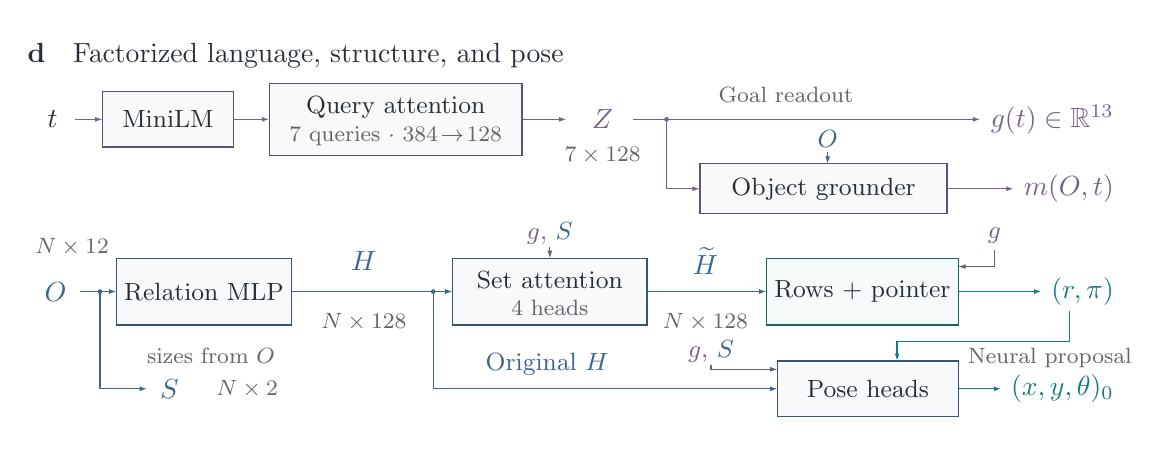
\begin{tikzpicture}[x=1bp,y=-1bp,line cap=butt,line join=miter]
\node[anchor=west,text=ink,font=\fontsize{10}{11.5}\selectfont,] at (0,10) {\textbf{d}\quad Factorized language, structure, and pose};
\node[anchor=center,text=ink,font=\fontsize{10}{11.5}\selectfont,] at (9,33) {$t$};
\draw[draw=violet,line width=0.5bp,-{Latex[length=2.7bp,width=1.8bp]}] (17,33) -- (27,33);
\path[fill=violet!4,draw=violet!70!ink,line width=.45bp] (27,23) rectangle (74,43);
\node[anchor=center,text=ink,font=\fontsize{9.4}{10.9}\selectfont,] at (50.5,33.0) {MiniLM};
\draw[draw=violet,line width=0.5bp,-{Latex[length=2.7bp,width=1.8bp]}] (74,33) -- (87,33);
\path[fill=violet!4,draw=violet!70!ink,line width=.45bp] (87,20) rectangle (178,46);
\node[anchor=center,text=ink,font=\fontsize{9.3}{10.8}\selectfont,] at (132.5,28.7) {Query attention};
\node[anchor=center,text=muted,font=\fontsize{7.9}{9.4}\selectfont,] at (132.5,39.0) {7 queries $\cdot$ $384\!\to\!128$};
\draw[draw=violet,line width=0.5bp,-{Latex[length=2.7bp,width=1.8bp]}] (178,33) -- (194,33);
\node[anchor=center,text=violet,font=\fontsize{10}{11.5}\selectfont,] at (207,33) {$Z$};
\node[anchor=center,text=muted,font=\fontsize{8}{9.5}\selectfont,] at (207,46) {$7\times128$};
\draw[draw=violet,line width=0.5bp,-{Latex[length=2.7bp,width=1.8bp]}] (218,33) -- (343,33);
\node[anchor=center,text=muted,font=\fontsize{8.5}{10.0}\selectfont,] at (273,24) {Goal readout};
\node[anchor=east,text=violet,font=\fontsize{10}{11.5}\selectfont,] at (391,33) {$g(t)\in\mathbb{R}^{13}$};
\fill[violet] (230,33) circle[radius=.85bp];
\draw[draw=violet,line width=0.5bp,-{Latex[length=2.7bp,width=1.8bp]}] (230,33) -- (230,58) -- (242,58);
\path[fill=violet!4,draw=violet!70!ink,line width=.45bp] (242,49) rectangle (331,67);
\node[anchor=center,text=ink,font=\fontsize{9.4}{10.9}\selectfont,] at (286.5,58.0) {Object grounder};
\node[anchor=center,text=blue,font=\fontsize{9.5}{11.0}\selectfont,] at (288,40) {$O$};
\draw[draw=blue,line width=0.45bp,-{Latex[length=2.7bp,width=1.8bp]}] (288,44.8) -- (288,49);
\draw[draw=violet,line width=0.5bp,-{Latex[length=2.7bp,width=1.8bp]}] (331,58) -- (355,58);
\node[anchor=east,text=violet,font=\fontsize{10}{11.5}\selectfont,] at (391,58) {$m(O,t)$};
\node[anchor=center,text=violet,font=\fontsize{9}{10.5}\selectfont,] at (188,74) {$g,\,{\color{blue}S}$};
\draw[draw=muted,line width=0.4bp,-{Latex[length=2.7bp,width=1.8bp]}] (188,79) -- (188,83);
\node[anchor=center,text=violet,font=\fontsize{9}{10.5}\selectfont,] at (348,75) {$g$};
\draw[draw=muted,line width=0.4bp,-{Latex[length=2.7bp,width=1.8bp]}] (348,80) -- (348,86) -- (335,86);
\node[anchor=center,text=muted,font=\fontsize{8}{9.5}\selectfont,] at (16,79) {$N\times12$};
\node[anchor=center,text=blue,font=\fontsize{10}{11.5}\selectfont,] at (10,95) {$O$};
\draw[draw=blue,line width=0.5bp,-{Latex[length=2.7bp,width=1.8bp]}] (19,95) -- (32,95);
\path[fill=blue!4,draw=blue!70!ink,line width=.45bp] (32,83) rectangle (95,107);
\node[anchor=center,text=ink,font=\fontsize{9.4}{10.9}\selectfont,] at (63.5,95.0) {Relation MLP};
\draw[draw=blue,line width=0.5bp,-{Latex[length=2.7bp,width=1.8bp]}] (95,95) -- (153,95);
\node[anchor=center,text=blue,font=\fontsize{10}{11.5}\selectfont,] at (121,84) {$H$};
\node[anchor=center,text=muted,font=\fontsize{8}{9.5}\selectfont,] at (121,106) {$N\times128$};
\path[fill=blue!4,draw=blue!70!ink,line width=.45bp] (153,83) rectangle (223,107);
\node[anchor=center,text=ink,font=\fontsize{9.3}{10.8}\selectfont,] at (188.0,90.7) {Set attention};
\node[anchor=center,text=muted,font=\fontsize{7.9}{9.4}\selectfont,] at (188.0,101.0) {4 heads};
\draw[draw=blue,line width=0.5bp,-{Latex[length=2.7bp,width=1.8bp]}] (223,95) -- (266,95);
\node[anchor=center,text=blue,font=\fontsize{10}{11.5}\selectfont,] at (244,84) {$\widetilde H$};
\node[anchor=center,text=muted,font=\fontsize{8}{9.5}\selectfont,] at (244,106) {$N\times128$};
\path[fill=teal!4,draw=teal!70!ink,line width=.45bp] (266,83) rectangle (335,107);
\node[anchor=center,text=ink,font=\fontsize{9.4}{10.9}\selectfont,] at (300.5,95.0) {Rows + pointer};
\draw[draw=teal,line width=0.5bp,-{Latex[length=2.7bp,width=1.8bp]}] (335,95) -- (365,95);
\node[anchor=east,text=teal,font=\fontsize{10}{11.5}\selectfont,] at (391,95) {$(r,\pi)$};
\fill[blue] (26,95) circle[radius=.85bp];
\draw[draw=blue,line width=0.5bp,-{Latex[length=2.7bp,width=1.8bp]}] (26,95) -- (26,130) -- (43,130);
\node[anchor=center,text=blue,font=\fontsize{10}{11.5}\selectfont,] at (51,130) {$S$};
\node[anchor=center,text=muted,font=\fontsize{8}{9.5}\selectfont,] at (79,130) {$N\times2$};
\node[anchor=center,text=muted,font=\fontsize{8}{9.5}\selectfont,] at (66,118) {sizes from $O$};
\fill[blue] (146,95) circle[radius=.85bp];
\draw[draw=blue,line width=0.5bp,-{Latex[length=2.7bp,width=1.8bp]}] (146,95) -- (146,130) -- (270,130);
\node[anchor=center,text=blue,font=\fontsize{9}{10.5}\selectfont,] at (187,121) {Original $H$};
\node[anchor=center,text=violet,font=\fontsize{9}{10.5}\selectfont,] at (246,116.5) {$g,\,{\color{blue}S}$};
\draw[draw=muted,line width=0.4bp,-{Latex[length=2.7bp,width=1.8bp]}] (246,121.5) -- (246,123) -- (270,123);
\path[fill=blue!4,draw=blue!70!ink,line width=.45bp] (270,120) rectangle (335,140);
\node[anchor=center,text=ink,font=\fontsize{9.4}{10.9}\selectfont,] at (302.5,130.0) {Pose heads};
\draw[draw=teal,line width=0.5bp,-{Latex[length=2.7bp,width=1.8bp]}] (375,102) -- (375,113) -- (313,113) -- (313,120);
\draw[draw=teal,line width=0.5bp,-{Latex[length=2.7bp,width=1.8bp]}] (335,130) -- (350.5,130);
\node[anchor=east,text=teal,font=\fontsize{10}{11.5}\selectfont,] at (391,130) {$(x,y,\theta)_0$};
\node[anchor=center,text=muted,font=\fontsize{7.6}{9.1}\selectfont,] at (368,119) {Neural proposal};
\pgfresetboundingbox
\path[use as bounding box] (0,0) rectangle (396,143);
\end{tikzpicture}
\end{document}
